\textit{This test was made together with Kjeld Jensen in order get one step further to spoofing the drones onboard GPS with an RTK GPS. A ublox Neo6-P GPS and an active <ANTENNE> was mounted on a EDUQuad drone to obtain the drone's position. A RPI was used on the EDUQuad to convert GPGGA and GPRMC from the Neo6-p GPS to CAN-mesasagess.
The test was done by walking 20 meters with the EduQuad two times to compare the output of the UKF with the different GPS's.
The values used to spoofed the GPS was found by analyzing a logfile from a regular flight to see the range of the values such as accuracy, DOP etc. when the drone was in the air. 
Values available from the Neo6-p GPS, was used directly to spoof the onboard GPS and values not available was either calculated or hardcoded.
Three tests were made due to a few code-errors but only the first and the last will be described. This test was also relevant for the indoor flying since the indoor application requires the position of the drone can be spoofed and the accuracies and DOPs can be set}\\

%\begin{wrapfigure}{r}{0.5\textwidth}
%  \begin{center}
\begin{figure}[H]
\centering
    \includegraphics[width=0.4\textwidth]	{graphics/eduquad_outdoor_flighttest_rpi_can_spoof.png}
	  \caption{Nep-6p connected to a M4 through a RPI}
    \label{fig:qground_station_dop}
\end{figure}
%  \end{wrapfigure}


In order to easily switch between the onboard GPS and the Neo-6P GPS during the test, a switch on the Spectrum DX9\footnote{\url{http://www.spektrumrc.com/Products/Default.aspx?ProdId=SPMR9900} last visited 21. Maj} was read in AutoQuad's firmware to decide which of the two GPS's data should be used. When a GPS update(time, position or velocity) is received from the onboard GPS, the struct showed in code \ref{code:gpsData_Struct} is filled in. \\


%\begin{wrapfigure}{r}{0.5\textwidth}
%  \begin{center}
\begin{lstlisting}[language = c++, caption = Quality checks added to discard bad positions, label=code:gpsData_Struct]
typedef struct {
	...
    double lat;
    double lon;
    float height;   // above mean sea level (m)
    float hAcc;     // horizontal accuracy est (m)
    float vAcc;     // vertical accuracy est (m)
    float velN;     // north velocity (m/s)
    float velE;     // east velocity (m/s)
    float velD;     // down velocity (m/s)
    float speed;    // ground speed (m/s)
    float heading;  // deg
    float sAcc;     // speed accuracy est (m/s)
    float cAcc;     // course accuracy est (deg)
    float pDOP;     // position Dilution of Precision
    float hDOP;
    float vDOP;
    float tDOP;
    float nDOP;
    float eDOP;
    float gDOP;

    //Used in GPS spoof
    uint8_t fix;
    uint8_t satellites;
    int out_cnt;

	...
} gpsStruct_t;
\end{lstlisting}
%  \end{center}
%  \end{wrapfigure}


In order to spoof the onboard GPS correctly, the author and his supervisor decided to overwrite all of the relevant elements in the struct. However, the RTC was set from the onboard GPS.

In order to know the required bytes to send latitude and longitude with a precision of 1 cm, the author used the datum WGS84\footnote{WGS-84 used in AQ} to estimate the worst-case error at equator. 

WGS-84 \footnote{\url{http://www.unoosa.org/pdf/icg/2012/template/WGS_84.pdf} last visited 22 maj} states that the semi-major-axis(a) of the earth is 6378137.0 m and that the flattening factor is 1/298.257223563. From these two values the semi-minor-axis(b) can be calculated using equation \ref{eq:raduis}
\begin{equation}
b=a \cdot (1-\frac{1}{298.257223563})
\end{equation} \label{eq:raduis}
Given the formula of the circumference of an ellipsoid:
\begin{equation}
circumference = 2 \cdot \pi \sqrt{ \frac{1}{2}(a^2+b^2)}
\end{equation} \label{eq:circum}
Equation \ref{eq:circum} gives a circumference at equator of 39873752.0 meters.

By dividing 39873752.0 by 360, one get how many meters pr. degree.
\begin{equation}
\frac{39873752.0}{360} = 110760 \frac{m}{deg}
\end{equation}

Table \ref{tab:precision_latlon} was made to see how many decimals is required to obtain different precisions.
\begin{table}[H]
\centering
\caption{Table shows precision required}
\label{tab:precision_latlon}
\begin{tabular}{@{}|l|l|l|@{}}
\toprule
Decimal place & Decimal degrees & Distance    \\ \midrule
0             & 1               & 110760 m    \\ \midrule
1             & 0.1             & 11076.0 m   \\ \midrule
...           & ..              & ...         \\ \midrule
7             & 0.0000001       & 7.75323 cm  \\ \midrule
8             & 0.00000001      & 0.775323 cm \\ \bottomrule
\end{tabular}
\end{table}

It can be seen that 8'th decimal is necessary to get below 1 cm. 
To see if a float can handle number smaller than $1\cdot e-8$, \textit{eps} from MatLab was used\footnote{http://se.mathworks.com/help/matlab/ref/eps.html}.
\begin{lstlisting}[language = matlab, caption = Check if float is precise enough of a double has to be used, label=code:eps_single]
eps(single(180.0)) = 1.5259e-05
eps(double(180.0)) = 2.8422e-14
\end{lstlisting}
In code \ref{code:eps_single} eps is given with 180 as input since 180 is the largest integer possible with using latitude and longitude.
It can be seen that the smallest number a float can represent is 1.5259e-05 but a precession of $1\cdot e-8$ is needed.
However a double can easily handle that which makes the latitude and longitude of the CAN-messages 8 bytes each. \\

2 bytes are allocated for each velocity, speed and heading. In order to send 2 decimals, each value was multiplied by 100 when sending and divided by 100 when received by AutoQuad.

Only one decimal for rest of the values was deemed necessary and was thereby multiplied and divided by 10. \\

To tell the UKF in AQ how much to believe in the GPS coordinates, the onboard GPS feeds the UKF with DOP factors. The DOP factors expresses how well the satellites are placed. If they are all located around the same spot, the DOP factors will be high since the triangulation becomes less accurate. The DOP factors has no unit but is simply a scaling of the error estimate. \cite{kelddueholmmikkellaurentziusannab.o.jensen2015}

\Mathias{Insert image from normal flight}
\newpage
Figure \ref{fig:dop_read_flight} shows a flight using onboard GPS where the DOP values where read. The values listed in table \ref{tab:DOP} was used and multiplied by the hDOP received from the Neo-6P GPS. 
\begin{wrapfigure}{r}{0.35\textwidth}
 \begin{center}
	\caption{Scaling factors used when using Neo-6p GPS}
	\label{tab:DOP}
	\begin{tabular}{@{}|l|l|@{}}
	\toprule
	Dop  & Value     \\ \midrule
	pDOP & 1.75*hdop \\ \midrule
	hDOP & 1*hdop    \\ \midrule
	vDOP & 1.5*hdop  \\ \midrule
	tDOP & 1.5*hdop  \\ \midrule
	nDOP & 0.7*hdop  \\ \midrule
	eDOP & 0.7*hdop  \\ \midrule
	gDOP & 1*hdop    \\ \bottomrule
	\end{tabular}
  \end{center}
\end{wrapfigure}

The pDOP was set to 1.75 times higher than the hDOP since it incorporates error from both vDOP and hDOP \cite{kelddueholmmikkellaurentziusannab.o.jensen2015}. \\
vDOP is usually 1.5-2 tims higher than hDOP.  \cite{kelddueholmmikkellaurentziusannab.o.jensen2015}. \\
tDOP was sat to 1.5 higher than hDOP since timeerror causes position error. \footnote{\url{http://www.environmental-studies.de/GPS/Dilution-of-precision/dilution-of-precision.html} last visited 22 maj} \\
Since hDOP can be split into nDOP and eDOP, they each of some of the error factor. \\
\Mathias{Gdop, skal den ikke være højere siden den har både vDOP, hDOP og tDOP} \cite{kelddueholmmikkellaurentziusannab.o.jensen2015}




\begin{figure}[H]
\centering
    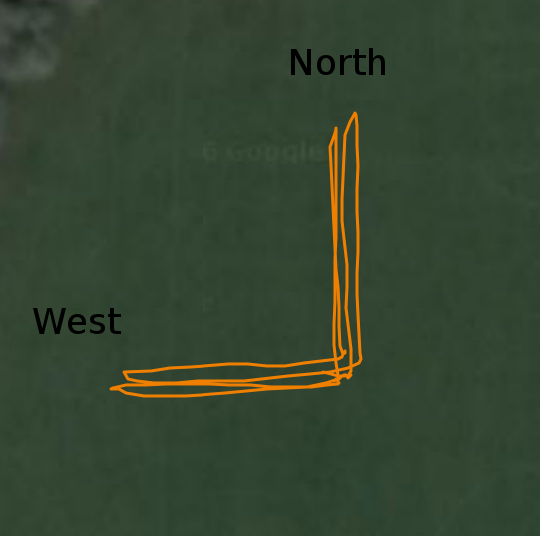
\includegraphics[width=0.4\textwidth]	{graphics/test_walked_90deg.png}
	  \caption{Path walked. If looking close it can be seen the path was walked twice, once with onboard GPS then using Neo-6p}
    \label{fig:qground_station_dop}
\end{figure}
The test was conducted by walking 20 meters \footnote{Measured by counting footsteps} north, 20 meters south, 20 meters east and 20 meters west. After walking 20 meters a small break of five seconds was held. Figure \ref{fig:position_plot} shows the walked path.
\Mathias{Figure med gpgga plot}
The coordinates plotted in figure \ref{fig:position_plot} was from the first test. Figure \ref{fig:ukf_plot} shows a plot of the position with x-axix as time.
\Mathias{Plot af northing and easting fra ukf}
Figure \ref{fig:ukf_plot} matches with the walked path seen in figure \ref{positon_plot}. The line crossing severel times is the switch on the Spectrum DX9 transmitter. It can be seen how the path repeats itself after the switch has been switched.
\Mathias{plot af pos og switch samt dop så man kan se de ændrer sig ved skift.}
Figure \ref{fig:ukf_dop} shows the same plot but where the vDOP and hDOP has been added. It can be seen when zoomed in, how the DOP values is also changing since the DOPs are higher when switching to the Neo-6p GPS.


\Mathias{Billede der viser højden/hastigheden er mere woobly siden DOP er mega lav, den stoler for meget på GPS}


Figur der viser højden samt højdehastigheden

figur der viser vele og veln der ikke virker.

Ny test, samme måde som første test, dog med følgende resultater \footnote{fejlen skyltes forkert blevev hevet ud fra C++ vector samt en variabel var brugt forkerte sted.}

\cite{kelddueholmmikkellaurentziusannab.o.jensen2015}





